%%
%% 第二章
%% 2012.5.20

\chapter{基于相似图像集的图像重建算法}

本文所使用的图像重建方法主要分为两个步骤,首先使用请求图像的局部特征在大规模数据集上进行相似图像的搜索,将搜索结果中最为相似的若干张图像作为重建候选图像集;其次,利用请求图像的局部特征在候选图像集上做更为精确的图像重建。本文将对两个技术层面分别加以阐述,本章探讨如何使用小规模候选图像集进行图像重建及其优化策略,下一章着重探讨大规模图像搜索领域中的相似图像搜索算法。

% 图像重建可以被概括的定义为这样一个基本问题:从一个退化版本的二维物体估算实际的二维物体\cite{Demoment:1989tw}。退化过程的数学形式取决于图像重建算法实际的应用场景。

% %%%%---------------------------------------传统的图像重建算法---------------------------------------------%%%%
% \section{传统的图像重建算法}
% 传统的图像图像重建算法所使用的场景一般是指图像修复(Image Restoration),原始“物体”由于经历了某种退化过程,不能直接由观测信息判断出来,为了消除退化过程的影响,必须根据观测到的数据进行重建来还原得到原始信息。
% 在图像修复中,引起退化的原因叫做失真,其定义如下:
% \begin{equation}
% y = A(X) \bullet b
% \end{equation}
% 其中\(A(\cdot)\)是退化函数,可以看做是一个滤波器,b表示的是噪声,\(\bullet\)表示的叠加方式。失真通常包含对X的卷积或者模糊,加性噪声或者乘性噪声。
% 而图像修复的解决方案是通过对观测信息进行退化模型的数学建模,利用约束条件来推导出退化过程的逆过程,对观测信息进行逆过程得到原始图像。

% 另一类图像重建场景是超分辨率重建,在近年来得到飞速的发展,是炙手可热的研究领域,它的基本思想是通过多张连续的低分辨率图像序列得到一张高分辨率的图像。很多数字图像应用中都需要高分辨率的图像,高分辨率的图像能够提供更佳的视觉体验,提供更丰富的信息,比如高分辨率的医学图像能够让医生更好的进行病情诊断,高分辨率的卫星图像能够进行更准确的模式识别任务。从1970年代以来,CCD和CMOS传感器被大规模的使用,获得了大量的数字图像,但是很多图像的分辨率较低,不能满足日益增长的业务需求,超分辨率重建是在这样的背景下诞生的\cite{Park:2003hg}。

% 那么,我们如何通过多张低分辨率图像获得一个高分辨率图像呢?如果一个场景下有多张低分辨率图像,而且这些图像从不同的角度来“描述”这个场景,那么这些低分辨率的图像可以看做是该场景的子采样和子像素精度的位移。如果这些低分辨率图像是以整数像素为单位进行的位移,那么多张低分辨率图像没有提供任何“新的信息”,但是如果位移单位是子像素单位的,序列中的每一个图像不能够由其他图像得出,换言之每个图像都提供了子像素精度的不同信息,我们可以利用这些信息重建一个高分辨率的图像。
% 一般来说,SRR算法分为基于重建和基于学习的两大类:基于重建的算法如频域重建法利用图像序列的交叠关系,凸集投影(POCS)等利用一些先验知识来约束求解过程,以达到增加细节信息的目的;基于学习的算法则使用多种机器学习的概率模型,包括基于流形学习、基于支持向量机和基于独立分量的超分辨率重建技术。基于学习的方法采用大量的高分辨率图像构造学习库来训练学习模型,在对低分辨率图像进行重建的过程中引入由学习模型获得的先验知识,进而得到图像的高频细节,获得较好的图像重建效果。

% 总体而言,超分辨率重建的整个流程包括三个基本环节:
% (1)低分辨图像的预处理,包括降噪和裁剪等基本图像数据处理。
% (2)配准过程,利用像素的空间信息估算低分辨率序列图像之间的运动矢量和空间位置关系。
% (3)完成重建,使用图像分割和融合等技术,利用多帧低分辨率图像的信息完成超分辨率重建。
%%%%-------------------------------------于局部特征的图像重建算法---------------------------------------------%%%%

本文所采用的图像重建的部分流程可以看成是多幅图像的全景图拼接问题。与文献\cite{Brown:2006ir}中的流程类似,主要包含以下几个环节:(1)使用具有不变性的特征来描述图像;(2)自动的找到图像之间的空间位置关系,进行图像配准;(3)图像融合,消除不同图像之间的光照差别,去除边缘噪声。与全景图拼接不同的是,本文使用的图像重建算法以图像块(Patch)作为拼接的最小单位,图像块像素数量分布不均匀、图像块之间有大量的重叠区域、图像块位置不够精确等特征点给拼接带来了一定的难度。本章从上述技术环节出发,分别探讨图像局部特征、特征匹配、图像配准等环节,并提出了针对图像块拼接的优化方案。

%%%%----------------------------------------局部特征---------------------------------------------%%%%
\section{图像的局部特征}

\subsection{局部特征概述}
图像的局部特征是计算机视觉领域一个基本问题,它能够反映图像某一局部的特性,对寻找图像对应的局部单元以及特征描述有着重要作用。通常意义的局部特征包含两个方面,特征检测子(Detector)和特征描述子(Descriptor)。检测子能够检测出我们“感兴趣”的点或者局部区域,而一个好的局部特征描述子反映出图像的局部特性能够帮助找到图像与图像点集合对应关系,进而建立图像之间的空间对应关系。局部图像特征描述的核心问题是不变性(invariant)和可区分性(discrimination)。

\begin{enumerate}
\item 不变性:指的同一局部特征经过不同的变换之后,仍然具有较强的相同特性,例如光照或透视产生变换后,同一描述子仍然能够被识别。
\item 可区分性:指的是描述不同局部特征的描述子有着较大的差别,可以被显著的区分。
\end{enumerate}

然而特征描述子的可区分性的强弱和其不变性是矛盾的,也就是说,一个具有诸多不变性的特征描述子,它区分图像局部内容的能力就稍弱;而一个非常容易区分不同图像局部内容的特征描述子,它的鲁棒性往往比较低。因此,在基于局部特征的图像处理中,研究不仅具有较强不变性、还具有较好区分性的特征描述子有着重要意义。

目前人们提出的众多图像局部特征算子中,由Lowe提出的尺度不变特征变换(Scale Invariant Feature Transform,简称SIFT)应用最为广泛。1999年首次提出,至2004年得到完善\cite{Lowe:2004uq}的SIFT算子是图像局部特征研究领域的一项重大突破。SIFT算子具有很强的可区分性,同时对尺度、旋转以及一定视角和光照变化等图像变化都具有不变性。在其之上衍生出来的SURF(Speeded Up Robust Features)是对SIFT的改进版本,它利用Haar小波来近似SIFT方法中的梯度操作,同时利用积分图技术进行快速计算,SURF的速度是SIFT的3-7倍。

除此以外,常见的特征检测子包括Harris角点,ANMS等,描述子还包括DAISY,ASIFT,MROGH,BRIEF等,分别适用于不同的图像应用场景下,本文提出的系统采用适用性最广泛的SIFT算子,下面我们对其进行简要的介绍。

\subsection{尺度不变特征变换}

(1)尺度空间理论

尺度空间理论是一个多尺度信号表示的框架,这一框架来源于物理学和生物视觉,被广泛用于计算机视觉、图像处理、信号处理领域。
尺度空间理论目的是模拟图像数据的多尺度特征。尺度空间中各尺度图像的模糊程度逐渐变大,能够模拟人在距离目标由近到远时目标在视网膜上的形成过程。我们将一幅图像按照尺度空间展开,第一层是原始图像,第二层是原始图像的模糊表示,第三层是第二层基础上的再次加以模糊,依次向上叠加,最上层可以抽象成一个像素点。可以看出,尺度空间上依次展开的图像构成了一个图像金字塔。当金字塔的层数足够多,每次模糊的值足够小的时候,我们认为尺度空间是连续的。
观察可以发现,金字塔的每一个截面与原图像相似,在实际的应用中,我们只取有限个截面构成离散的尺度空间上的值。因此金字塔的步长越小,层数越多,特征描述越精确,但处理时间会相应增加;层数太少会导致粒度过于粗糙,下采样的截面中可能找不到尺寸大小一致的两个物体的图像。一个图像的尺度空间\(L(x,y,\sigma)\)定义为一个变化尺度的高斯函数\(G(x,y,\sigma)\)与原图像\(I(x,y)\)的卷积。
\begin{equation}
  L(x,y,\sigma) = G(x,y,\sigma) \otimes I(x,y)
\end{equation}

其中
\begin{equation}
  G(x,y,\sigma) = \frac{1}{2\pi\sigma^2}e^{-\frac{(x-m/2)^2+(y-n/2)^2}{2\sigma ^2}}
\end{equation}
这里m,n表示高斯模板的维度,\((x,y)\)表示像素点的位置。\(\sigma\)是空间尺度因子,决定了图像在尺度空间上的哪一个位置,也是高斯平滑的参数,它的值越小,图像被平滑的程度越小,尺度越小。

高斯金字塔的构建方式如图\ref{fig:pyramid}所示

\begin{figure}
\centering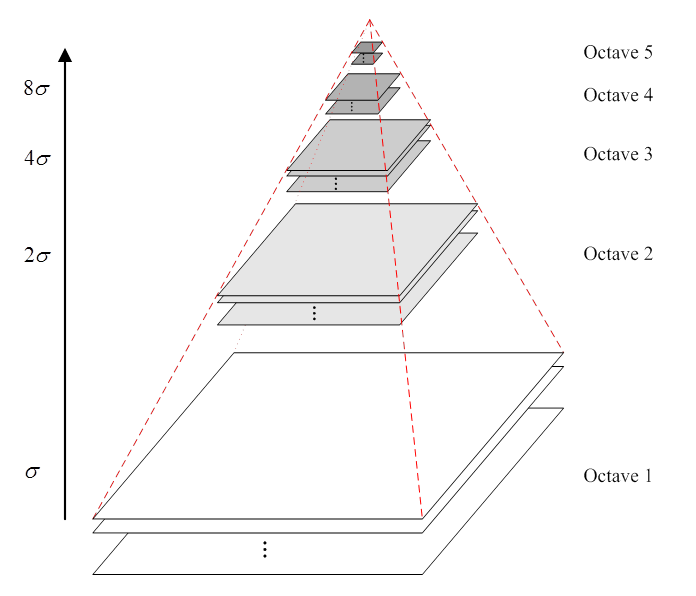
\includegraphics[width=15cm]{imgs/ch2/pyramid}
\caption{金字塔模型的生成}
\label{fig:DoG}
\end{figure}

将原始图像不断降阶采样 ,得到一系列大小不一的图像 ,由大到小,从下到上构成的塔状模型。原图像为金子塔的第一层 ,每次降采样所得到的新图像为金字塔的一层(每层一张图像),每个金字塔共n层。金字塔的层数根据图像的原始大小和塔顶图像的大小共同决定。

为了让尺度体现其连续性,高斯金字塔在简单降采样的基础上加上了高斯滤波。将图像金字塔每层的一张图像使用不同参数σ做高斯模糊,使得金字塔的每层含有多张高斯模糊图像,将金字塔每层多张图像合称为一组(Octave),金字塔每层只有一组图像,组数和金字塔层数相等。

图\ref{fig:DoG}反映了图像金字塔的情况:

\begin{figure}
\centering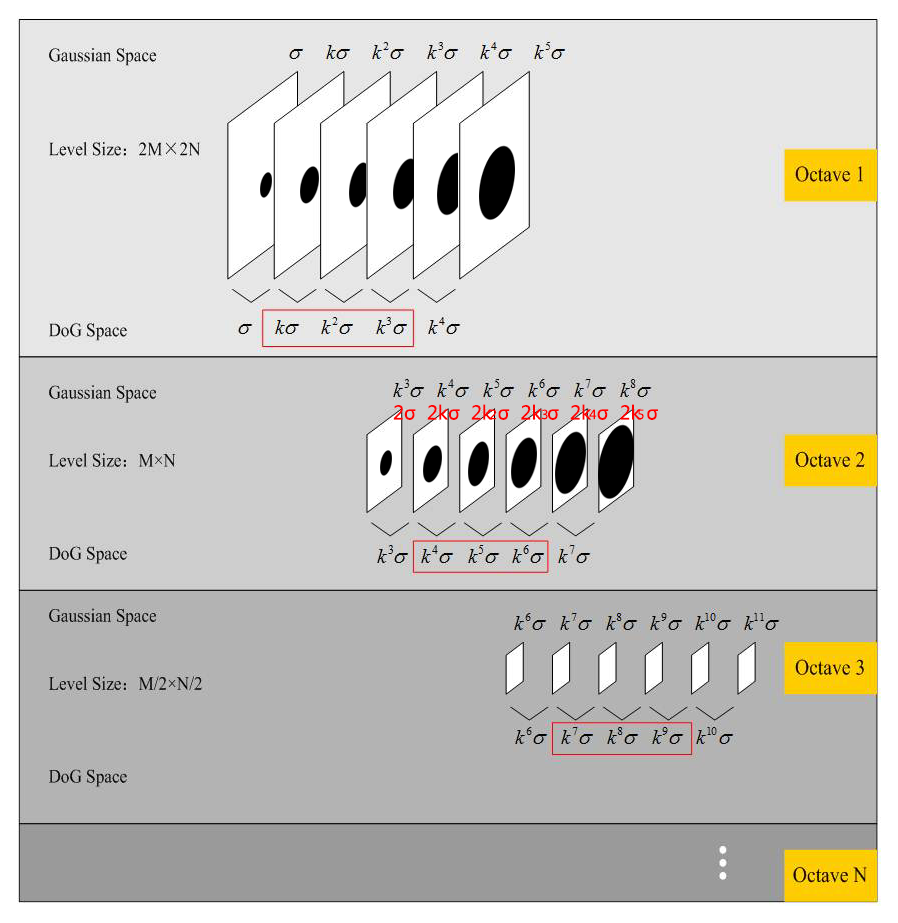
\includegraphics[width=15cm]{imgs/ch2/DoG}
\caption{金字塔图像空间关系}
\label{fig:DoG}
\end{figure}

图中的黑色圆盘表示的是该图像所在的尺度的特征覆盖的范围,其特点是不同组同一层上的特征覆盖范围一样,同一组不同层上的特征覆盖范围逐步增大。关键点的尺度坐标就是按关键点所在的组和组内的层,利用下面这个公式计算而来:
\begin{equation}
  \sigma(o,s) = \sigma_0 2^{o+s/S},
  \quad o \in o_{\min} + [0, ..., O-1],
  \quad s \in [0,...,S-1]
\end{equation}

(2)SIFT检测子

SIFT算法有两个主要环节,一个是检测“感兴趣”的关键点,另一个是描述这个“关键点”。SIFT关键点是精心选择的一组在高斯差分尺度空间(Difference of Gaussians scale space,DoG)上的极值点,该关键点包含三个关键信息,分别是(1)亚像素精度的(x,y)位置信息;(2)尺度大小,反映关键点在局部的影响范围,决定了特征的覆盖区域像素数量,对后文局部图像块的提取起到至关重要的作用;(3)所在高斯尺度空间上的主方向,该主方向是由一个高斯窗口函数计算得来,反映的是关键点所在局部的方向信息。其中差分高斯尺度空间表示为
\begin{equation}
  D(x,\sigma(s,o)) \doteq G(x,\sigma(s+1,o)) - G(x,\sigma(s,o)).
\end{equation}

其中\(σ\)表示尺度空间坐标,\(O\)表示组(octave)数,\(S\)表示组内层数,\(σ_0\)是基准层尺度,\(o\)为组的索引,\(s\)为组内层的索引。关于尺度空间和描述子的具体讲解在Lowe的论文中\cite{Lowe:2004uq}已有详细的介绍,这里不再详述。

(3)SIFT描述子

SIFT描述子反映关键点局部的信息,是高斯尺度空间上某一局部和方向上的梯度信息,以直方图的形式对信息做统计,最终每一个描述子是一个128的特征。

%%%%----------------------------------------匹配--------------------------------------------%%%%
\section{特征匹配}
提取图像的局部特征之后,我们希望找到两幅相似的图像间相一致的特征点,这一过程叫做特征匹配。匹配环节最重要的两个步骤是匹配策略的确定和高效的数据结构以及相应的匹配算法。

\subsection{匹配策略}
如果已知一个SIFT描述子和其它所有描述子的相似程度的数值表示,则可以采取如下的匹配策略:
\begin{equation}
  M(S,S_r) = 
\begin{cases} 
\text{true}, & \mbox{if } S_r = S_{min},\frac{\text{Dis}(S,S_{min})}{\text{Dis}(S,\tilde{S}_{min})} > C \\
\text{false}, & \mbox{otherwise}
\end{cases}
\end{equation}

\(S\)是待匹配的描述子,\(S_r\)是所有候选描述子中的一个,\(S_r = S_{min}\)说明\(S_r\)是与待匹配描述子最为接近的一个。\(\text{Dis}(\cdot,\cdot)\)表示的是两个特征描述子之间的相似性度量,比如可以用欧氏距离表示,距离越大,相似性越小。\(S_{min}\)和\(\tilde{S}_{min}\)分别表示的是与S距离最近和第二近的特征。而C是一个阈值常数,通常取1.5。上式表明,如果最匹配的特征的距离比其次匹配特征的距离的比值大于一定的程度,则认为该特征有最佳匹配,最佳匹配就是最为相似的特征;如果比值小于阈值,则认为匹配失败。

\subsection{高效匹配算法}
能实行上述匹配策略的前提条件是:“能够在较短的时间内比较当前特征点和每一个候选特征点的相似性,进而找到最为相似的一个候选特征。”在解决这个最近邻问题时,总体的时间复杂度是\(O(n^2)\),在大多数的应用中使用并不现实。因此我们需要找到更为合适的索引结构来存储数据,进行快速的查找。解决这种高维数据查询检索的一些常见算法包括使用多维散列,局部敏感哈希(Locality Sensitive Hashing)以及多维搜索树等。本文使用多维搜索树中最为常见的k-d树(K-dimension tree),下面对其做简要介绍。

k-d树是一种空间划分树,它把整个特征空间交替沿着垂直于坐标轴的超平面将空间进行分割,分割时尽量使得特征点的分布保持平衡。然后在特定的划分内进行相关搜索操作,有效减少搜索范围。

构建k-d树遵循如下的规则:

(1)随着树的深度增加,循环的选取坐标轴,作为分割超平面的法向量。对于维度为3的树来说来说,根节点选取x轴,根节点的孩子选取y轴,根节点的孙子选取z轴,根节点的曾孙子选取x轴,这样循环下去。

(2)每次均为所有对应实例的中位数的实例作为切分点,切分点作为父节点,左右两侧为划分的作为左右两子树。

对于n个实例的k维数据来说,建立k-d树的时间复杂度为O(k*n*logn)。

k-d树的搜索算法如下\cite{李航2012统计学习方法}:
\begin{enumerate}
\item 在k-d树种找出包含目标点x的叶子节点:从根节点出发,递归访问k-d树。若x当前维的坐标小于切分点的坐标,则移动到左子结点,否则移动到右子节点。直到叶子节点。
\item 以当前叶子节点为“当前最近点”。
\item 回溯:递归的回退,对每个节点:

	\begin{itemize}
	\item 如果该节点比当前最近节点离目标更近,则更新“当前最近点”
	\item 当前最近点一定存在于该节点某个子节点对应的区域,检查该子节点的兄弟节点对应的区域是否有更近的点。
	\end{itemize}

\item 回退到根节点,结束,“当前最近点”即为最近邻特征点。
\end{enumerate}
%%%%----------------------------------------配准--------------------------------------------%%%%
\section{图像配准}

在得到两幅图像(在本文中是两个图像块)相匹配的特征点之后,我们有了相对应点的位置关系,如何利用这些位置关系将两幅图像重合的部分放置于正确的位置上,是本节讨论的议题。

\subsection{直接变换法}
根据两个图像块的位置、方向、尺度直接写出两个图像块之间的变换公式,称作直接法,本节首先介绍各种2D变换,最后介绍如何根据匹配图像块的空间信息直接写出变换矩阵。

(1)旋转和平移变换,也叫2D刚体运动即2D欧式变换(因其保持欧式距离),写作\(x={Rx+t}\)或者写作
\begin{equation}
	x' = 
	\begin{bmatrix}
	R & t	
	\end{bmatrix}
	\bar{x}
\end{equation}
其中
\begin{equation}
	R = 
	\begin{bmatrix}
	\cos{\theta} & -\sin{\theta} \\
	\sin{\theta} & \cos{\theta}
	\end{bmatrix}
\end{equation}
是一个正交旋转矩阵,有\(RR^T = I\)和\(|R| = 1\)

(2)放缩旋转,也叫做相似变换,该变换可以表示为\({\bar{x}}={sRx+t}\),其中s是一个任意的尺度因子。它也可以写作
\begin{equation}
	x ={ 
	\begin{bmatrix}
	sR & t
	\end{bmatrix}
	\bar{x}
	}
	={
	\begin{bmatrix}
	a & -b & t_x \\
	b & a & t_y
	\end{bmatrix}
	\bar{x}
	}
\end{equation}
其中\(a^2 + b^2 = 1\)这一约束条件不再需要。相似变换前后,直线间的夹角保持不变。

各种2D变换如表\ref{2dtrans}所示。

\begin{table}[h]
\caption{2D坐标变换}
\label{2dtrans}
\centering
\begin{tabular}{|c|c|c|c|}
\hline
\textbf{变换} & \textbf{矩阵大小} & \textbf{自由度数} & \textbf{保持} \\ \hline
平移          &   \(2\times{3}\)	& 2             & 方向          \\ \hline
刚性(欧式)    &   \(2\times{3}\) & 3             & 长度          \\ \hline
相似          &   \(2\times{3}\)  & 4             & 夹角          \\ \hline
仿射          &   \(2\times{3}\)  & 6             & 平行性         \\ \hline
投影          &   \(2\times{3}\)   & 8             & 直线性         \\ \hline
\end{tabular}
\end{table}


使用SIFT算法得到匹配到的特征点后,可以根据一对匹配的SIFT算子直接写出两个图像块的变换矩阵,称该变换为\(H_0\),具体求解方式如下:

结合一对匹配SIFT特征点\(\tilde{S}\)和\(S\)的位置\(\tilde{x}_f,x_f\)、尺度\(\tilde{s}_f},{s_f}\)和方向\(\tilde{\theta},\theta)\),可以得到两个图像块\(P_{\tilde{S}}\)和\(P_S\)的变换矩阵\(H_0\):

\begin{equation}
	H_0 = 
	\begin{bmatrix}
	\frac{\tilde{s}_f}{s_f} R & T
	\end{bmatrix}
\end{equation}
其中
\begin{equation}
	R = 
	\begin{bmatrix}
		\cos{(\tilde{\theta}-\theta)} & -\sin{(\tilde{\theta}-\theta)} \\
		\sin{(\tilde{\theta}-\theta)} & \cos{(\tilde{\theta}-\theta)} 
	\end{bmatrix}
\end{equation}

\begin{equation}
	T = 
	\begin{bmatrix}
		\tilde{x}_f - x_f \\
		\tilde{y}_f - y_f
	\end{bmatrix}
\end{equation}

下面介绍如何使用随机抽样一致算法求解\(H\)。

\subsection{随机抽样一致算法}
随机抽样一致(RANdom SAmple Consensus,RANSAC)是一种空间匹配算法。该算法将数据分成两类,局内点(inlier)和局外点(outlier)它可以从一组包含局外点的观测数据集中,通过迭代方式估计数学模型的参数。

这是一种不确定的算法,有一定的概率得出一个正确的或者说是可接受的合理结果;一般情况下,迭代次数的增加可以提升结果的准确性。该算法由Fischler和Bolles于1981年提出,在图像检索中,RANSAC可以作为检索后的后续处理,对图像中的目标进行空间一致验证。

RANSAC算法对数据集做了三个假设:

\begin{enumerate}
\item 数据由局内点组成,局内点的数据的分布符合某一特定的概率模型;
\item 与局内点相对的是局外点,他们不能够适应该模型;
\end{enumerate}

RANSAC有以下几个步骤:
\begin{enumerate}
\item 随机选择数据集合的一个子集;
\item 使用所选择的子集拟合出一个数学模型;
\item 确定该模型下局外点的个数;
\item 重复步骤1~3若干次,以最好的一次结果最为最终拟合出来的数学模型。
\end{enumerate}

RANSAC算法迭代次数的选取取决于期望的准确率与样本数量。设p为任意给定对应点合法的概率,即
\[p = \frac{\text{局内点的数量}}{\text{数据集全部数据的数量}}\]
而\(P\)是经过S次试验后成功的总体概率。设需要k个随机样本来估计模型,那么在一次试验中,该k个样本都是局内点的可能性为\(p^k\)。因此,S次试验失败的可能性是
\[1 - P = (1 - p^k)^S\]
两边去对数,得到最少需要的试验次数是
\[S = \frac{log(1-P)}{log(1-p^k)}\]
随着k的增大,需要的最少试验次数增多,在实际中,应该尽可能的选择小的k值。在模型确定以及最大迭代次数允许的情况下,RANSAC总是能找到最优解。对于含有较大误差的数据集,RANSAC的效果远优于直接的最小二乘法。

当对两幅图像进行匹配的时候,所以相互匹配的局部特征作为数据全集,待估算的模型是一个变换矩阵H,能够将图像\(I\)投影到图像\(I'\)。每次迭代过程中,随机的选择四对匹配的特征点,根据这四个特征点的位置信息解得变换H,利用H计算其它匹配对的位置信息中有哪些属于局外点,记录局外点的个数。局外点的个数越少,变换矩阵H越准确。反复迭代多次得到一个相对准确的透视变换模型。

上述提到的用四对匹配点拟合出的变换矩阵叫做单应矩阵(Homography),最简单的求解单应性矩阵的算法叫做直接线性变换法(Direct Linear Transform,DLT)\cite{Dubrofsky:2009tz},其具体算法如下:

假设相匹配的一对点分别是\(x\)和\(x'\),单应性矩阵是\(H\),那么有如下等式:

\begin{equation}
\label{homography1}
	c
	\begin{pmatrix}
	u \\
	v \\
	1
	\end{pmatrix}
	= H
	\begin{pmatrix}
	x \\
	y \\
	1
	\end{pmatrix}
\end{equation}


其中c是一个非零常数,\((u\ v\ 1)^\mathrm{T}\)代表\(x'\),\((x \ y \ 1)^\mathrm{T}\)代表\(x\),而
\(
H = 
\begin{pmatrix}
h_1 & h_2 & h_3 \\
h_4 & h_5 & h_6 \\
h_7 & h_8 & h_9
\end{pmatrix}
\)

将公式\eqref{homography1}展开,分别用第一行和第二行除以第三行,得到

\begin{equation}
\label{homography2}
-h_1x - h_2y - h_3 + (h_7x+h_8y+h_9)u = 0
\end{equation}

\begin{equation}
\label{homography3}
-h_4x - h_5y - h_6 + (h_7x+h_8y+h_9)u = 0
\end{equation}

公式\eqref{homography2}和\eqref{homography3}可以写成矩阵的形式:
\begin{equation}
\label{homography4}
A_ih = 0
\end{equation}

其中
\(A_i = 
\begin{pmatrix}
-x & -y & -1 & 0 & 0 & 0 &ux & uy & u \\
0 & 0 & 0 & -x & -y & -1 &vx & vy & v 
\end{pmatrix}\)
,而
\(h = (h_1 \ \ h_2 \ \ h_3 \ \ h_4 \ \ h_5 \ \ h_6 \ \ h_7 \ \ h_8 \ \ h_9)^\mathrm{T}\)。
因为每一对匹配的点可以提供两个等式,对于解决8自由度的矩阵H,只需要四对(任意三点不能共线)匹配的特征点。

DLT算法依赖于坐标系的原点和尺度,所以该算法并不稳定,在实际中更多的使用多个匹配点得到更多的方程,将求单应矩阵的问题转化为求解最小二乘的问题,用矩阵奇异值分解(Singular value decomposition,SVD)的方法来求解等式\(Ah = 0\)。

计算出的\(H_0\)和\(H\)都可以作为块的旋转矩阵,在实际的系统中,会同时计算两个矩阵,比较他们的准确程度,挑选使用准确度高的变换矩阵。比较的准则一般使用2D变换后的图像块与其相应位置的上采样图像的均方误差作为验证标准,在实际中,按照一定的规则只接受符合要求的图像块,具体的规则将在下一节中介绍。

%-----------------------------------------自己的内容,自适应阈值的图像块筛选法----------------------------------------
\section{图像块筛选法及其改进算法}
\subsection{人工设定阈值法}
到目前为止,已经得到了每个原图像特征对应的候选图像块并将其通过变换矩阵H变换到相匹配的位置上。因为每个图像块有其自身的方向、尺度、位置,图像块之间可能存在交叠,其中有些图像块与原图在像素值上存在较大的出入,需要利用上采样图像计算配准后的图像块与原图像块的误差,根据设定好的阈值\(\epsilon\)移除误差较大的图像块。

原图像经过特征提取、过滤操作后,有几百个大尺度图像块,在分布密集区域,图像块有大量的重叠,并不需要对每一个候选图像块做最后的拼接。利用相似图像搜索得到候选图像,在候选图像中利用特征匹配找到原图像块匹配的候选图像块,虽然在SIFT描述子级别上两个候选图像块是匹配的,但无法保证像素级别上的一致。

在文献\cite{Dai:2012vn}中,使用上采样图像\(I_u\)来校验候选图像块是否正确。校验规则为是

\begin{align}
\label{eq:errorControl}
  \text{Verify}(P_{\tilde{S}}) = 
\begin{cases} 
\text{true}, & \mbox{if MSE} (T(P_{\tilde{S}}),P_c \in I_u) < \epsilon \\
\text{false}, & \mbox{otherwise}
\end{cases}
\end{align}

其中\(\text{MSE}(\cdot,\cdot)\)表示的是两个图像块的均方误差(Mean Square Error)。\(T(P_{\tilde{S}}\)表示对候选图像块进行透视变换,\(P_{S}\)是\(P_{\tilde{S}}\)经过透视变换后在\(I_u\)上的相匹配区域。\(\epsilon\)表示一个阈值常数,当两个图像块的均方误差大于一个阈值时,判定为该图像块匹配失败,否则认为是正确匹配。这里的难点是误差阈值\(\epsilon\)的确定,阈值设定过大,错误匹配块无法筛掉,阈值设定太小,筛选掉相对准确的匹配块,导致最后拼合有缺陷。一般情况下根据经验人为的指定一个相对合理的阈值。

实验结果显示认为指定阈值的方式往往不能泛化到一般请求图像上,因此本文提出了一种自适应阈值的图像块筛选法,将在下一节介绍。

\subsection{自适应阈值的图像块筛选法}

我们发现在公式\ref{eq:errorControl}中,因为\(I_u\)是由原始图像经过下采样、编解码、再上采样得到,上采样图像与原始图像在各个区块本身包含了误差,而且误差的大小与每一幅特定的图像以及图像的降采样和插值方式有关。如果设定一个固定的阈值,对于有些请求图像来说,可能会筛掉正确的块,对于另一些请求图像,可能会保留错误的匹配块。

针对上述出现的阈值设置的难题,本文设计了一种在基于客户端预处理的阈值自适应的方法,能够根据请求图像的不同动态的调整验证阈值。

实验发现,原始图像高频区域的图像块经过降采样再插值后得到的图像块与原始像素值有了较大的区别,平滑区域图像块经过降采样和插值处理后像素值的整体变化较小,有着较小的误差。又因为原始图像和候选图像在局部区域上往往是角度、透视的变换,在像素值的梯度场的变化两者是一致的,所以原始图像与上采样图像的误差也反映了候选图像与上采样图像之间的误差。

有些原始图像整体较为平滑,与\(I_u\)误差不大,能够较好的反映原图的像素信息,这类使用较低的误差阈值能够得到较好的重建效果,与此相反,有些图像整体或者局部包含大量高频信息,图像\(I_u\)经过了平滑处理在像素信息上有了较大的损失,再使用小的阈值会导致误筛掉正确的匹配块。
自适应阈值方法在客户端计算每一个原始图像块上,计算每一个图像块在上采样图像块和原始图像块上的均方误差,在所有的均方误差数值中选取一个适当的值作为基准误差,再根据服务器端匹配的候选区块数量加上一定的宽容度。

自适应阈值方法的步骤是:
\begin{enumerate}
\item 提取图像\(I\)的SIFT算子,保留其中大于指定尺度的SIFT算子
\item 对原始图像\(I\)进行降采样、编码、解码、上采样,得到\(I_u\)
\item 计算每一个SIFT算子对应的图像块\(P_S\)
\item 计算每一个图像块在\(I\)和\(I_u\)上的均方误差,找到其中最大的作为基准误差\(\epsilon_b\)
\item 在服务器端利用候选相似图像几何做SIFT匹配得到匹配块,根据匹配块的数量M,计算宽容度\(\frac{\epsilon_C}{M}\)
\item 得到最终的验证误差阈值为:
\begin{align}
\epsilon = \epsilon_b + \frac{\epsilon_C}{M}
\end{align}
\end{enumerate}

其中\(\epsilon_C\)为一常数,\(\frac{\epsilon_C}{M}\)的意义是当匹配图像块数量较少时,容许的宽容度增大,尽量保证匹配的图像块能够作为重建图像的一部分,当候选图像块较多时,宽容度变小,重建条件变得苛刻。在步骤四找基准误差时,可以比较最大值与第二大的数值之间的差值,如果过大,说明最大值可能是异常点,可以将其移除后重复步骤四。
%-------------------------------------结束----------------------------------------

\section{图像分割}

得到较为精确的候选图像块后,会发现图像的部分区域是不正确的,我们希望将图像块做进一步的划分,根据图像分割算法将图像切割成若干块,找到其中误差较大的块移除。本文主要采用的是基于图的图像分割算法\cite{Felzenszwalb:2004il}。

\subsection{图像分割与感知重要性理论}

图像分割的在很多应用中非常重要,是很多高层应用的前提,比如识别、索引等。我们认为图像分割的方法应该满足如下特性:
\begin{itemize}
\item 能够捕捉到感知上比较重要的区域。这通常体现在图像的全局特性方面,一方面要提供感知重要的精准属性,另一方面能够确定给定的分割技术的使用场景。对分割结果属性有精确定义的方法易于理解,便于与其他的方法进行比较。
\item 高效,接近线性时间复杂度。为了能够实际使用,分割方法应该与边缘检测或者其他底层图像处理技术有着相似的时间复杂度,即处理时间与像素数量成线性关系,而且常系数也比较小。每一秒能对几帧图像进行分割的算法就能够处理实时的视频数据。
\end{itemize}

本文采用了\cite{Felzenszwalb:2004il}提到的图像分割算法,在保证效率的同时考虑到了图像全局属性上的感知重要区域。

\begin{figure}
\centering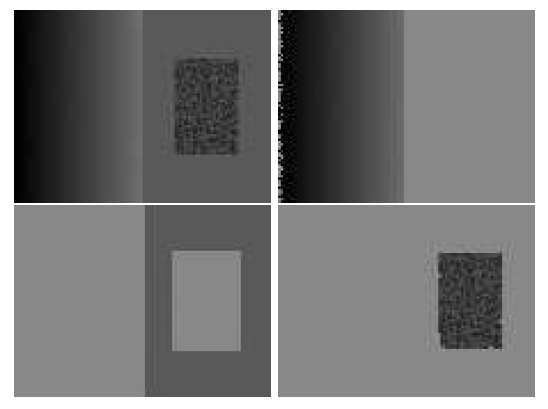
\includegraphics[width=15cm]{imgs/ch2/man_made}
\caption{人造图像}
\label{fig:man_made}
\end{figure}
首先我们来看图\ref{fig:man_made}所示的人造图像,这个例子能够解释什么是感知重要属性(conceptually important property)。人眼会认为这幅图像有三个区域,如左下角图像所示,右边两幅图像是采用两种分割策略产生的分割结果。这个例子能够说明:(1)全局的亮度的变化不应该单独的作为分割区域的衡量标准。比如图像中左侧渐变区域和右侧的高频噪声区域都有较大的亮度变化,但是我们他们应该被分割成多个区域。因此,假设一个区域有着接近恒定的亮度是不正确的。(2)区域划分不能单纯的依靠局部划分标准。例如图中渐变图像与常量区域的边界上的亮度差值比很多高频区域的差值要小,因此我们得出结论,为了分割一幅图像,需要引入一些非局部衡量标准。

因此,本文提出的衡量标准将会比较两个属性:
\begin{itemize}
\item 边界的亮度差值
\item 区域内部的邻居像素间的亮度差值
\end{itemize}
我们认为,两个区域的边界上的亮度差值如果比比两个区域中至少一个区域的内部像素差值大的话,那么边界亮度差值会更多的影响人们的感知,这个时候边界亮度差是感知重要的。

\subsection{基于图的图像表示}

这一节探讨如何使用图的方式来表示图像。

令\(G=(V,E)\)表示一个无向图,点集\(v_i \in V\),待分割的元素集合。边\((v_i,v_j) \in E\)有一个相应的权重\(w((v_i,v_j))\),是一个非负值,描述两个相邻元素\(v_i\)和\(v_j\)的不相似度。在图像分割领域,V中的元素就是像素点,边是两个像素点(这两个像素点是相邻的)不相似性的某种度量(例如亮度,颜色,运动,位置或者其他局部属性)。这里的公式和不相似性度量的方法是独立的,可以按照自己的需求定制度量方案,这里讨论的是大框架。

在基于图的方法中,一个分割方案S是V的一个划分,每一个区域\(C \in S\)对应着图
\(G' = (V,E')\)的一个连通区域,其中\(E' \subseteq E\)。有许多方法来衡量一个分割的好坏,大体上我们希望\textbf{一个区域内部的元素尽可能相似,不同区域之间的像素尽可能不同}。这意味着同一区域内,相邻两个点的有相对来说比较小的权值,不同区域的相邻两个点的边有大的权值。

\subsection{内部不相似度与外部不相似度}

这一节我们讨论分割区域的衡量标准。

首先定义一个预测D,来估计是否存在一个显著的证据表明有一个边界能将两个区域分割开。就像上文说的,就是对外部的不相似性与内部不相似进行比较,也就是比较内部相似和外部相似的差值。

接下来定义内部不相似性为该区域最小生成树的最大边,\(MST(C,E)\),即:
\begin{equation}
Int(C) = \mathop {\max }\limits_{e \in MST(C,E)}w(e)
\end{equation}

可以容易推断出该方法保持连通的最低要求是Int(C)这个边所决定的。

我们定义两个区域的差异为:区域\(C_1,C_2 \subseteq V\),连接这两个区域的所有边的权值中,最小的那个权值。即,
\begin{equation}
Dif(C_1,C_2) = \mathop {\min }\limits_{v_i \in C_1 ,v_j \in C_2, (v_i,v_j) \in E}w((v_i,v_j))
\end{equation}

如果两个区域没有连接的边,则令\(Dif(C_1,C_2) = \infty\)

区域比较预测法通过比较\(Dif(C_1,C_2)\)和\(Int(C_1)\)与\(Int(C_2)\)中较小的一个,来判断这两个区域是否有一个边界,也就是判断这两个区域是否有足够的理由保持两个区域。

\begin{equation}
f(n) =\begin{cases} 
true,   \mbox {if } \mbox Dif(C_1,C_2) > M Int(C_1,C_2)\\\\
false,  otherwise \end{cases}
\end{equation}

下面引入一个阈值函数来控制我们希望的外部不相似度与内部不相似度的相差程度。
\begin{equation}
MInt(C_1,C_2) = min(Int(C_1) + \tau(C_1),Int(C_2) + \tau(C_2))
\end{equation}
对于比较小的区域,\(Int(C)\)并不能够较好的反应局部特性,比如最极端的情况下,当\(|C| = 1\)时,\(Int(C) = 0\)。因此我们需要一个跟区域大小相关的阈值函数
\[\tau (C) = \frac{k}{|C|}\]
其中\(|C|\)表示的是区域C的大小,k是一个常数。越是小的区域,我们越希望较大的外部不相似性。
在实际中可以调整k的取整来获得不同的效果。当k值很大时,算法倾向于分割出来较大的块,当k值较小时,算法倾向于更细的划分。

\(\tau\)函数的选取是决定了分割的倾向性,如果我们改变这个函数,不会对算法的大框架造成影响,而会对分割结果的倾向性有影响。比如我们可以让分割倾向于某一种形状A,令\(\tau\)函数在区域不是形状A的时候较大即可。这种形状上的倾向可以比较简单,比如希望正方形的或者扁平状的,也可以比较复杂,是一种特殊的形状。

\subsection{分割算法}

本节讲解主要的算法部分,怎样利用上述的定义,在基于图的表示方法下,做出高效而准确的分割。算法的输入是一个图\(G=(V,E)\),有n个点和m个边。输出是一个分割V,分割成\(S=(C_1,...,C_2).\)。算法流程如下:

\begin{enumerate}
\item 对E进行排序,生成非递减的序列\(\pi = (o_1,...,o_m)\)
\item 从初始分割\(S^0\)开始,每一个点\(v_i\)自己就是一个区域
\item 对于每一个\(q = 1,...,m\)执行步骤4
\item 通过\(S^{q-1}\)构建\(S^q\),使用如下的方式:令\(v_i\)和\(v_j\)表示按顺序排列的第q条边的两个点,比如\(o_q = (v_i,v_j)\)。如果\(v_i\)和\(v_j\)在\(S^{q-1}\)中连个不同的区域下,并且\(w(o_q)\)比两个区域的内部不相似度都小,那么合并这连个区域,否则什么也不做。用公式来表达就是:令\(C_{i}^{q-1}\)是\(S^{q-1}\)的一个区域,它包含点\(v_i\);令\(C_{j}^{q-1}\)是\(S^{q-1}\)的一个区域,它包含点\(v_j\)。如果\(C_{i}^{q-1} \neq C_{j}^{q-1}\)并且\(w(o_q) \leq MInt(C_i^{q-1},C_j^{q-1})\),那么通过合并\(C_{i}^{q-1}\)和\(C_{j}^{q-1}\)我们得到了\(S^q\);否则的话\(S^q = S^{q-1}\)
\item 返回\(S = S^m\)
\end{enumerate}

按照上述流程,最终得到的分割结果如图\ref{fig:segment}所示,得到了较满意的效果。
\begin{figure}
\centering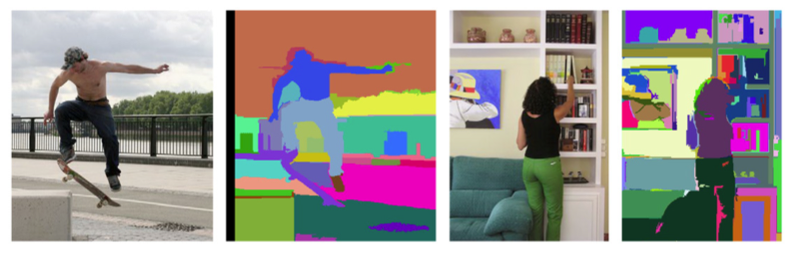
\includegraphics[width=15cm]{imgs/ch2/segment}
\caption{基于图的图像分割结果}
\label{fig:segment}
\end{figure}

%%%%----------------------------------------融合--------------------------------------------%%%%
\section{图像融合}

图像融合是指将多幅包含相关信息的图像处理成一幅图像的过程。相比于每一幅输入图像,输出图像往往包含了更丰富的信息。图像融合方法大体上可分为两类,一类是空间域融合,另一类是变换域融合。

经过图像配准之后,不同的图像经过2D变换,变换到正确的位置上。对于某些重合区域的像素来说,该位置上有两个或多个以上的像素,图像融合问题就是利用怎样的规则求得这些位置上的像素的值。常见的有取均值法,Brovey方法,主成分分析法以及基于高频率波法,IHS和基于曲波变换等技术。

在本文的图像重建系统中,图像融合是重建部分的最后一步,本文的图像融合有这样几个特点:

\begin{enumerate}
\item 待融合的图像块数很多,通常在几十到几百个;
\item 图像块的大小跨度很大,小的块有几十个像素,大的块有上万个像素;
\item 因为融合之前对每一个图像块进行了分割,所以图像块并不一定是完整的,融合的可能是块的一部分区域;
\item 有一张原图像的下采样图像作为参考图像,为图像融合提供了可靠的依据
\end{enumerate}

通过观察上述四个特点我们发现,如果我们以下采样图像作为第一块拼合图像,采用图像块由大到小的方式依次拼接,那么图像融合的任务转变成逐一将小图像块贴合在一个背景图像上,是一个典型的图像无缝拼接任务,解决这个问题的经典方案是泊松图像编辑。

\subsection{泊松图像编辑}
泊松图像编辑是一种自动的“无缝融合”两张图像的技术,在文献\cite{Perez:2003ul}中首次提出。该方法所用的数学工具是带狄里克雷边界条件的泊松偏微分方程,狄里克雷边界条件指定了在影响域内未知函数的拉普拉斯算子,以及在区域边界上的未知函数值的拉普拉斯算子\cite{张建桥:2010vm}。

需要解决的问题定义如下:需要被改变的图像是\(S\)(称为背景图像),我们剪切粘贴的图像是\(g\)(称为前景图像)。两幅图像的位置关系如图\ref{fig:poi_dis}所示。

\begin{figure}
\centering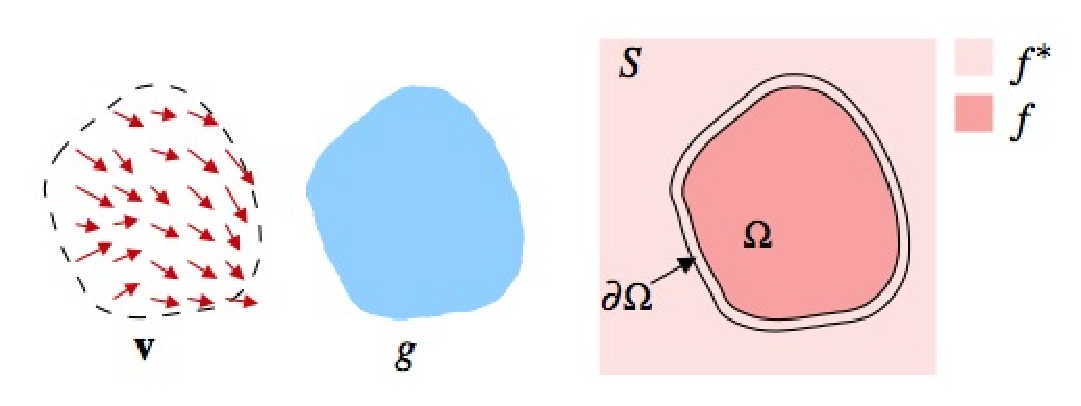
\includegraphics[width=8.00cm]{imgs/ch2/poi_dis}
\caption{泊松图像编辑区域示意图}
\label{fig:poi_dis}
\end{figure}

两幅图像融合的标准时:允许图像g改变颜色,但是仍然能够保留g的完整的“细节”。细节包括g中的边缘、角点、过度等等。而从图像中提取这些细节的多种方法中,都会使用到\textbf{图像梯度}。图像梯度是描述图像的一种数学表达,描述的是像素与相邻像素的相对变化(本质上是像素与其相邻像素的差值)。我们需要寻找的就是相对描述子,因为图像A与图像B之间的不统一主要是因为他们颜色上的绝对差。因此,更为严格的泊松图像编辑的目标是:允许改变绝对信息,即图像B的颜色,但是在粘贴之后尽可能的保留B的相对信息,即图像梯度。

我们将图像g的边缘像素固定,其像素值为图像S的像素值,然后求解其余的在选取内的像素值,约束条件是保持图像g的原始梯度。

设对g进行校正后得到的图像是f,f能够更好的与S融合。g的边界与S的边界完全一致,匹配选取内部的像素,向内融合:

\begin{equation}
f_{(x,y)} = S_{(x,y)}\forall{(x,y)}\in{\partial{f^*}}
\end{equation}
其中\(\partial{f^*}\)表示\(f^*\)的边界

我们期望g内部像素的梯度值等于S内部像素的梯度值。一个点上图像梯度的定义是:该像素与所有像素的差值的和
\begin{equation}
|\nabla{f^*_{(x,y)}}| = 4f^*(x,y) - f^*(x-1,y) - f^*(x+1,y) - f^*(x,y-1) - f^*(x,y+1)
\end{equation}

我们需要解决的问题是一个求最小值的问题:
\begin{equation}
\mathop {min}\limits_{f}\iint_{\Omega}^{} |\nabla{f}|^2\text{ with }f|_{\partial\Omega} = f^*|_{\partial\Omega}
\label{fusion_problem}
\end{equation}
这个求最小的问题满足欧拉-拉格朗日(Euler-Lagrange)等式:
\begin{equation}
\Delta f = 0\text{ over }\Omega\text{ with }f|_\partial{\Omega} = f^*|_\partial{\Omega}
\label{eul-lag}
\end{equation}

其中\(\Delta = \frac{\partial^2.}{\partial{x^2}}+\frac{\partial^2.}{\partial{y^2}}\)是拉普拉斯算子,公式\eqref{eul-lag}是满足Dirichlet边界条件的拉普拉斯等式。
我们将公式\eqref{fusion_problem}稍加修改,引入一个引导域\(v\),得到如下结果:
\begin{equation}
\mathop {min}\limits_{f}\iint_{\Omega}^{} |\nabla{f} - v|^2\text{ with }f|_{\partial\Omega} = f^*|_{\partial\Omega}
\label{fusion_problem2}
\end{equation}

公式\eqref{fusion_problem2}的解是满足狄利克雷边界条件的泊松等式:
\begin{equation}
\Delta f = div\mathbf{v}\text{ over }\Omega\text{ with }f|\partial{\Omega} = f^*|\partial{\Omega}
\label{poi_equ}
\end{equation}
其中\(div\mathbf{v} = \frac{\partial u}{\partial x}+\frac{\partial v}{\partial y}\)是\(\mathbf{v} = (u,v)\)的散度。

上式等效于求
\begin{equation}
\Delta \tilde{f} = 0\text{ over }\Omega,\tilde{f}|\partial{\Omega} = (f^* - g)|\partial{\Omega}
\label{poi_equ}
\end{equation}

其中\(f = g + \tilde{f}\),我们的问题转变成求差值的问题。

\subsection{泊松图像编辑离散解}
如果一个相邻像素是(1)边界像素,那么它的值是固定的;(2)超出选区边界,被排除。下面的差分方程总结了每一个像素点的所有情况
\begin{equation}
\begin{aligned}
|N|f(x,y) - \mathop {\Sigma }\limits_{(dx,dy)+(x,y) \in{\Omega}}f(x+dx,y+dy)
-\mathop {\Sigma }\limits_{(dx,dy)+(x,y) \in{\partial{\Omega}}}A(x+dx,y+dy) \\
= \mathop {\Sigma }\limits_{(dx,dy)+(x,y) \in{\Omega \bigcup {\partial{\Omega}}}}
f^*(x+dx,y+dy) - f^*(x,y)
\end{aligned}
\end{equation}

其中\((x,y)\)是2D网格上感兴趣的像素点的位置。N是相邻像素的数量(包含边界像素,N<=4)。\(\Omega\)是B选区(不包含边界),\(\partial \Omega\) 是边界,\((dx, dy)\)是可能的相邻像素点位置,包括 {(-1, 0), (1, 0), (0, -1), (0, 1)}。

等式左侧是计算未知像素点\(f(x, y)\)的空间梯度,计算的方式是将\(f(x,y)\)与每一个相邻的像素点做差值,并加和。每一个差值的形式都是\(f(x,y) - other(x',y')\),其中\((x',y')\)是其他像素点的位置。

等式右侧计算\(f^*\)图像在(x,y)处的梯度值,它与我们新的图像\(f\)的像素值匹配。

对于RGB图像,这些公式会分别处理R,G,B三个通道。

下一步需要为H中的每一个点列出等式,注意到这里列出了一组线性方程,包含k个未知数,k是需要求解的H中像素数量,最直接的方案是把所有的方程放到一个矩阵中,然后反转矩阵。然而,k的值相当的大,对于200X200的选取而言,k是40000。反转一个40000X40000的矩阵计算复杂度过高。

注意到矩阵是极为稀疏且正定的,因为每一个点至多有4个相邻像素,每一行至多有5个非零的元素,其余是0。针对这样的特性,可以采用迭代矩阵求解算法。使用Jacobi方法来求解稀疏线性方程组。Jacobi 方法是梯度下降算法的一个特例。它的基本思路是:

\begin{itemize}
\item 以\(A x = b\)的形式建立矩阵等式。A是上述定义的等式的矩阵,x是待求解的值,b是等式需要等于的值。
\item 初始化x,使之全为0;
\item 计算\(Ax\)的积;
\item 计算\(b-Ax\)的差值,这个差值衡量的是当前猜测的x的值和正确值之间的误差;
\item 将差值\((b-Ax)\)追加到x上。这就是我们让猜测向着正确方向前进的“梯度下降”的步骤;
\item 重复步骤3-5,直到x和\((b-Ax)\)之间的差值足够小;
\end{itemize}

因为A是正定的,这个过程能够保证收敛到x的正确的解,并以指数速度收敛。

\subsection{卷积近似解法}
解等式\eqref{poi_equ}需要多次迭代,耗费大量时间,文献\cite{Farbman:2011dc}使用薄膜插值法(Membrane Interpolation)。\(f^*\)的值可以通过近似方法得到,其思路是沿着区域边界平滑的拓展差值,直到展开到整个区域。差值可以写成卷积的形式:
\begin{equation}
\tilde{f} = \frac{G * \tilde{r}}{G * \tilde{R}}
\label{con_pyr}
\end{equation}
其中
\begin{equation}
\begin{cases} 
\tilde{r}(x_i) = f^*(x_i) - g(x_i), & \forall{x_i} \in \partial\Omega \\
0, & \mbox{其它}
\end{cases}
\label{con_pyr}
\end{equation}
而\(\tilde{R}\)是\(\tilde{r}\)的特征函数,\(G(x_i,x_j)\)是平移不变格林函数:
\begin{equation}
G(x_i,x_j) = G(\|x_i - x_j\|) = 2\pi\log{\frac{1}{\|x_i - x_j\|}}
\end{equation}
卷积可以通过三个个滤波器进行快速的计算,这个计算的时间复杂度是O(n),与像素数量呈线性关系。实验表明采用卷积近似解泊松方程得到的解的像素值和采用迭代求解差异不大,适用于本文的图像融合的场景下。


%% 本章参考文献
\ifx\usechapbib\empty
\nocite{BSTcontrol}
\bibliographystyle{buptgraduatethesis}
\bibliography{bare_thesis}
\fi